%
% File acl2020.tex
%
%% Based on the style files for ACL 2020, which were
%% Based on the style files for ACL 2018, NAACL 2018/19, which were
%% Based on the style files for ACL-2015, with some improvements
%%  taken from the NAACL-2016 style
%% Based on the style files for ACL-2014, which were, in turn,
%% based on ACL-2013, ACL-2012, ACL-2011, ACL-2010, ACL-IJCNLP-2009,
%% EACL-2009, IJCNLP-2008...
%% Based on the style files for EACL 2006 by 
%%e.agirre@ehu.es or Sergi.Balari@uab.es
%% and that of ACL 08 by Joakim Nivre and Noah Smith

\documentclass[11pt,a4paper]{article}
\usepackage[hyperref]{acl2020}
\usepackage{times}
\usepackage{latexsym}
\usepackage{graphicx}
\usepackage{amsmath}
\usepackage{amssymb}
\renewcommand{\UrlFont}{\ttfamily\small}

% This is not strictly necessary, and may be commented out,
% but it will improve the layout of the manuscript,
% and will typically save some space.
\usepackage{microtype}

%\aclfinalcopy % Uncomment this line for the final submission
%\def\aclpaperid{***} %  Enter the acl Paper ID here

%\setlength\titlebox{5cm}
% You can expand the titlebox if you need extra space
% to show all the authors. Please do not make the titlebox
% smaller than 5cm (the original size); we will check this
% in the camera-ready version and ask you to change it back.

\newcommand\BibTeX{B\textsc{ib}\TeX}

\title{Sentiment Classification of News Articles and Macroeconomics Prediction with Sentiment Scores}

\author{Siu-Hang Chan \\
  \texttt{chansiuhang@hotmail.com} \\\And
  Mustafa Panbiharwala \\
  \texttt{mustafa.shabbir10@gmail.com} \\}

\date{}

\begin{document}
\maketitle
\begin{abstract}
Abstract Pending
\end{abstract}

\section{Introduction}

Macroeconomics forecasting, e.g. economic growth, inflation, and unemployment rate, is one of the major tasks in macroeconomics, and it matters a lot for policymaker market participants. Traditionally, various economics factors are used as independent variables / features, e.g. survey data, for forecasting, most probably with an autoregressive model.

The recent advance in natural language technology and text analytics techniques have made the use of text information more practical on a large scale. As a result, researchers and market practitioners are looking into whether large text corpus, e.g. those from newspapers, can be helpful in macroeconomics forecasting or not.

Here, we will test if the hypothesis: text corpus from news articles are helpful in macroeconomics forecasting, is true or not. We expect the sentiment scores, which are estimated from text corpus from new articles using our own-trained sentiment classification model, will boost the prediction accuracy of the variables of concern.

In the following, we aim to build a pipeline that extracts information from news articles to help make assessments about the USA's economics (namely the GDP, CPI and unemployment rate). There will be two main steps there: 1) extract sentiment scores from unstructured news articles 2) using the sentiment scores to forecast a macroeconomic indicator such as Inflation or growth in the USA. For step (1), we plan to build a sentiment classification model using labelled data (text passage with labelled sentiment), and then use it on a larger unlabelled news dataset to construct a time series of sentiment scores. For step (2), the constructed time series of sentiment scores will be applied to forecasting of macroeconomic indicators and various models will be compared.


\section{Related Work}

There are various literatures about using text information for macroeconomics forecasting. While they have the same goal of assessing how sentiments extracted from the unstructured business news can be used to forecast macroeconomic indicators of a country's health, each of them have a slightly different approach in how they collect news data, how they create a sentiment analysis model and finally how they use the model to forecast the macroeconomic indicator.

There are different ways to construct the sentiment score. All papers use a lexicon based model for the task of sentiment analysis on news data. For example, in \cite{P1} \cite{P3} \cite{P4} \cite{P5} use predefined lexicons and human judgement to create daily sentiment scores across all business news articles and \cite{P7} used a Bi-LSTM model trained on a knowledge graph to extract sentiment scores.A completely different approach of skipping the sentiment score is also investigated in \cite{P6}.

The data source varies quite a lot too. Some of them are based on US newspapers \cite{P1} \cite{P3}, some on UK ones \cite{P6}, while \cite{P7} are based on a global database (GDELT). This shows that text information can be used to improve macroeconomics forecasts regardless of the location of the economy. Majority of the papers use a proprietary data source to extract news articles. \cite{P5} uses Dow Jones Newswires Archives to extract news articles from 1990 to 2016 and \cite{P4} uses LexsNexis’ proprietary smart indexing technology to extract news articles as well as topics associated with those articles. 

While considering the macroeconomics forecasting part, the most common benchmark is some form of autoregressive linear time series model, like the one used in \cite{P1} and \cite{P7}. Some other machine learning approaches like Lasso, Ridge, Neural Networks, SVM, and Random Forest are also discussed in \cite{P6}. A dynamic factor model approach is tested in \cite{P4} and \cite{P5} which uses dimensionality reduction technique on the sentiment scores generated from the text data to forecast the macroeconomic indicators. Also, although both \cite{P4} and \cite{P5} use to create sentiment scores for certain news topics, the way they extract these topics are very different. \cite{P5} use LDA on unstructured news data to extract and create their own news topics whereas \cite{P4} uses built in topics from their data source and skips this step of topic modeling. But both of the papers stress on the fact that sentiment scores based on news topics do have a high predictive power to forecast macroeconomic indicators.



\section{Data}

In this project, three dataset have been used in different steps:

\subsection{Financial Phrase Bank}


\subsection{Global Database of Events, Language, and Tone (GDELT)}

GDELT version 1.0, from 1-Apr-2013 to 30-Sept-2021, totally 3101 days of news are used for calculating the sentiment score. In this database, news on the web from all around the world is collected, but for the purpose of predicting macroeconomics variables of the United States, only US news is filtered for processing.

In the GDELT database, the URL of the website of each news item is stored in a CSV table, which contains the news of the same date. In order to read the text in the news, we first unzip the zip file that contains the CSV file, and then load the URL one by one to get the text in the news from the website. Unfortunately, this process is quite slow, and thus we can only sample some of the news each day due to time constraints of the project.
	

\subsection{Macroeconomics Data from FRED}

Three macroeconomics variables are of concern: GDP, CPI and Unemployment Rate, which are important ones that reflect the status of economic growth, price level, and the job market. The corresponding data from Federal Reserve Economic Data (FRED) are downloaded from Federal Reserve Bank of St. Louis: Real Gross Domestic Product (from Q1-1947, quarterly), Consumer Price Index for All Urban Consumers: All Items in U.S. City Average (from Jan-1913, monthly) and Unemployment Rate (from Jan-1948, monthly). In order to make the performance comparable between the model with sentiment scores calculated using GDELT, only the data from Apr-2013 / Q2-2013 to Sep-2021 / Q3-2021 is used.


\section{Sentiment Classification}

In order to estimate the sentiment of a piece of text, we build sentiment classification models based on a labeled database, where the Financial Phrase Bank is used for this purpose. This not only allows calculation of sentiment score of other news for various purposes, but also shows how good the built sentiment classification models are by themselves.


\subsection{Models}


\subsection{Experiment}


\subsection{Results and Analysis}


\section{Macroeconomics Forecasting}

In order to investigate if the text information from newspapers are useful in macroeconomics forecasting, we leverage the GDELT, and estimate the sentiment from the US news. Various sentiment scores are then constructed based on this, and they will be tested if they are statistically significant in macroeconomics variable construction.

\begin{table*}
\begin{center}
\begin{tabular}{|l|c|c|c|}
\hline
  & Unemployment & GDP & CPI\\
\hline\hline
ACF & 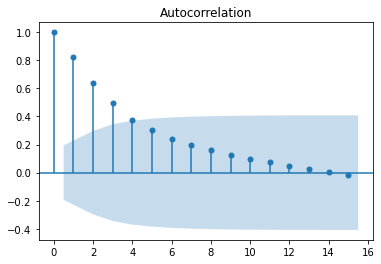
\includegraphics[width=40mm,scale=0.5]{images/ACF1.png} & 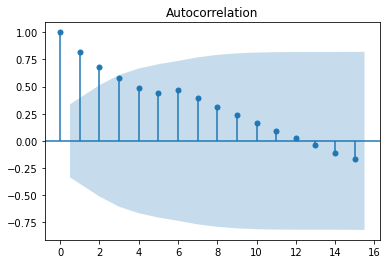
\includegraphics[width=40mm,scale=0.5]{images/ACF2.png} & 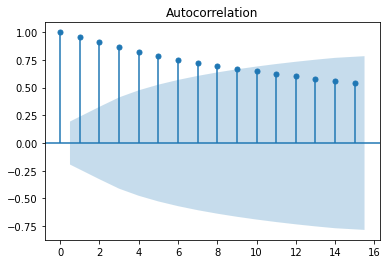
\includegraphics[width=40mm,scale=0.5]{images/ACF3.png}\\
\hline
PACF & 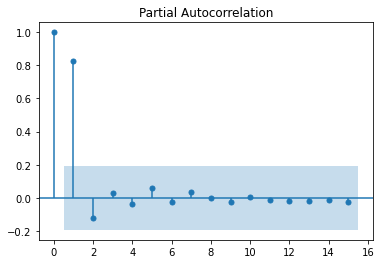
\includegraphics[width=40mm,scale=0.5]{images/PACF1.png} & 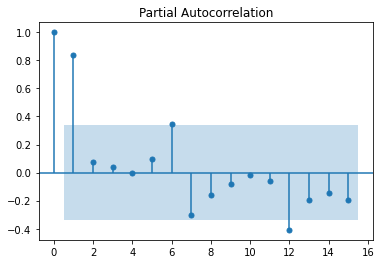
\includegraphics[width=40mm,scale=0.5]{images/PACF2.png}& 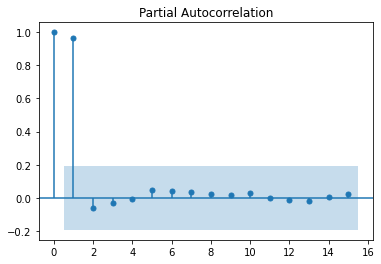
\includegraphics[width=40mm,scale=0.5]{images/PACF3.png}\\
\hline
\end{tabular}
\end{center}
\caption{ACT and PACF graph for macroeconomics variables}
\label{tab:acf_pacf}
\end{table*}


\begin{figure*}
\centering
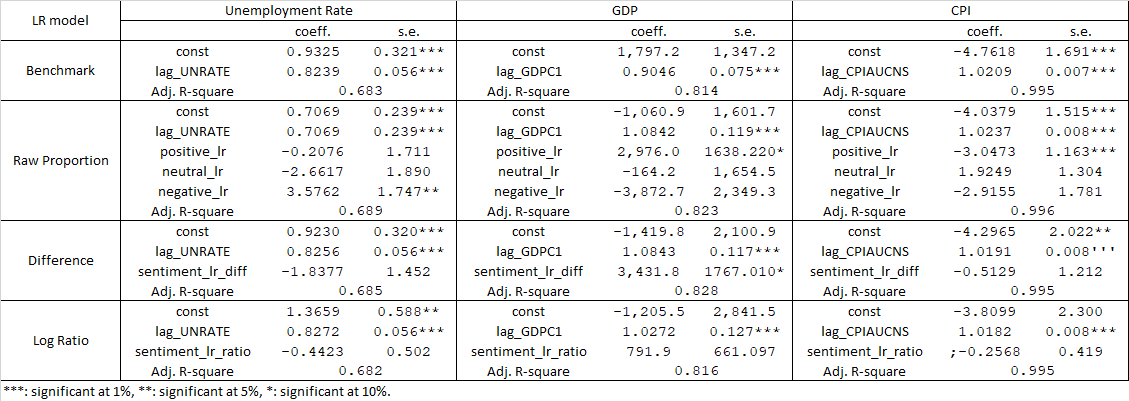
\includegraphics[width=150mm]{images/table_lr.png}
\caption{Regression from Benchmark model, and Model with Sentiment (under LR model)}
\label{fig_lr}
\end{figure*}

\begin{figure*}
\centering
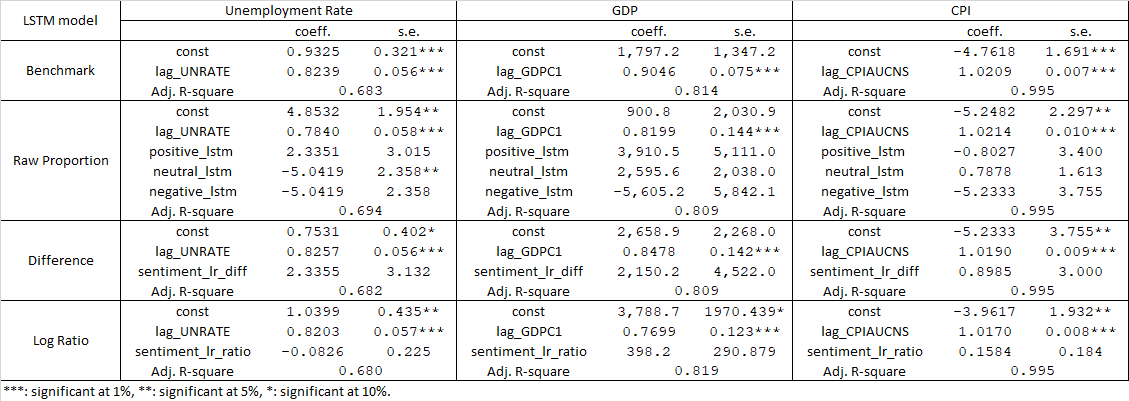
\includegraphics[width=150mm]{images/table_lstm.png}
\caption{Regression from Benchmark model, and Model with Sentiment (under LSTM model)}
\label{fig_lstm}
\end{figure*}

\subsection{Models}

Firstly, for each news, the sentiment is estimated by the sentiment classification models (LR and Bi-LSTM model respectively), and they are classified to positive, neutral and negative. For each month, the total number of positive, neutral, and negative news are counted, and the proportional of that are stored. We have computed three sentiment scores: the raw proportion of positive, neutral and negative news, the difference between positive and negative news, and the log of the ratio between the proportion of positive and negative news.

Secondly, the scores are added into the benchmark model one by one to see if they are statistically significant for prediction of the macroeconomics model. Due to autocorrelation in the three macroeconomics variables, an autoregressive similar to that adopted in \cite{P6} is used. Based on the ACF and PACF graphs, an AR(1) model is used as the benchmark to be compared with.






\subsection{Experiment}

Totally three baseline models are fitted, one for each of the GDP, CPI and unemployment. In addition, for each of the 3 macroeconomics variables, and for each of the 2 sentiment classification models (LR and LSTM), 3 linear models are trained for each method of the sentiment scores: the raw sentiment proportion, the difference, and the log ratio respectively, are trained, which make up to a total of 18 models.

Benchmark Model:

y_t = \alpha + \beta * y_{t-1} + \epsilon

with Sentiment Scores:

y_t = \alpha + \beta_1 * y_{t-1} + \beta_2 * sentiment_t + \epsilon

where yt is the macreconomics variable of concern at time t.

In order to conclude if the sentiment scores are useful or not, we check if the coefficients are statistically significant or not, and  check if the adjusted R-square are improved or not.


\subsection{Results and Analysis}

From the table below, we can see that the results are positive for most macroeconomics variables: namely the proportion of negative news are significant in prediction of unemployment rate, the proportion of positive news are strongly significant in prediction of CPI, and the proportion of positive news are weakly significant in prediction of GDP. In all cases, the adjusted R-square has also been improved.

[TABLES]

Comparing the models, it seems that the more simple LR model is performing slightly better than the more complicated LSTM one in macroeconomics forecasting. This can be the effect of better generalization to other dataset of a more simple model, or simply because of the way of how the sentiment scores are constructed.

While among the various ways of sentiment scoring, it seems that the raw proportion is the best among the three, possible due to the fact that it preserves the most information among them.



\section{Conclusion, Limitation and Further Work}

We have successfully built two sentiment classification models that predict the sentiment of news articles well. In addition, we have also found that the sentiment score calculated can be useful in predicting the unemployment rate and CPI, and also potentially useful for predicting the GDP.

As mentioned before, the sentiment scoring part is done on a sampling of the subset of the database due to time constraint, and the result can be more reliable if we can skip this sampling step. In addition, since the US economy can be affected by news in other countries, it will be also worth testing if including news elsewhere will help too.

Lastly, in the macroeconomics forecasting part, it would be contributive to test if other statistical model, e.g. Lasso, Ridge, Decision Tree will perform better too, just like what \cite{P6} did.


\bibliography{xcs224u_report}
\bibliographystyle{acl_natbib}

\end{document}
